% IPP
% Projekt - 1.
% Juraj Holub
% xholub40@stud.fit.vutbr.cz

\documentclass[a4paper, 10pt]{article}
\usepackage[utf8]{inputenc}
\usepackage[english]{babel}
\usepackage[T1]{fontenc}
\usepackage[left=2cm,top=2.5cm, right=2cm]{geometry}
\usepackage{hyperref}
\usepackage{graphicx}
\usepackage{float}

\title{Documentation of Project Implementation for IPP 2018/2019 }
\author{Name and surname: Juraj Holub\\ Login: xholub40}
\date{}

\begin{document}
	\maketitle
	\thispagestyle{empty}

% introduction
% proposal of solution
\section{Proposal of solution} \label{proposal}
Scheme of project solution is split into three blocks. 

The first block split input string to tokens representation where one token represents atomic lexeme of input programming language IPPcode19. The token is implemented like data structure with two attributes. The first attribute is the identification of token, for example, keywords or integer constant. The second attribute is the value of token specified by his identification, as an example, an integer constant contains a specific integer value.

The second block is a finite state machine (FSM). FSM input is a string of tokens and machine verify lexical and syntactical correctness of input program.

Third and last block is a generator of output in eXtensible Markup Language (XML). 

\begin{figure}[H] 
	\centering
	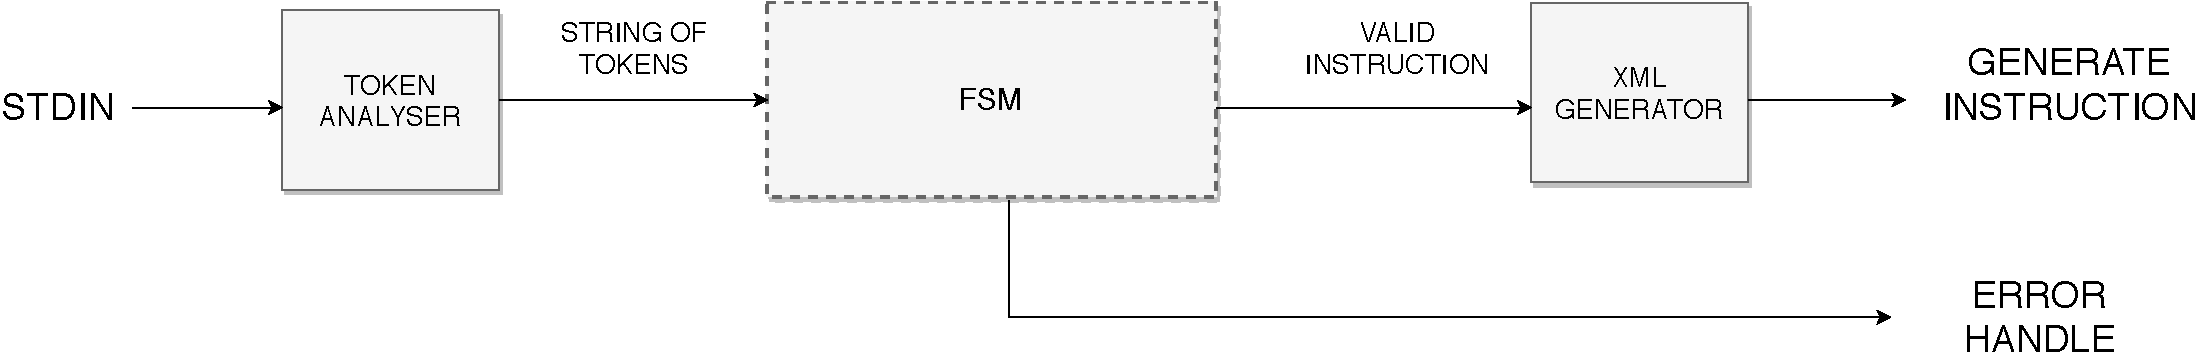
\includegraphics[width=.8 \paperwidth]{ipp_parse}
	\caption{Scheme of implemented parse solution.}
	\label{obr1}
\end{figure} 

Figure \ref{obr1} shows scheme of implemented algorithm of parsing IPPcode19 and generating XML output.

\section{Implementation details}
Suggested solution parted to three blocks described in section \ref{proposal} is implemented in three logical units:
\begin{itemize}
	\item \textbf{Tokens analyser}: Analyse input string from standard input of program char by char and convert them to the token representation. Supported tokens are instruction code, symbol, label, variable, type, white space and new line. Instruction codes are sorted to groups by number and types of arguments. Comments are ignored and token analyser skips them in input program string.
	\item \textbf{Parse}: Implementation of the finite state machine. FSM input is an actual token received from the token analyser. Machine output depends on the current state and current token which lead to Mealy FSM. If the input is valid then after every successive analyse of one IPPcode19 instruction is this instruction sends to XML generator. Incorrect input leads to error state where FSM read rest of tokens and then inform about an error.
	\item \textbf{XML generator}: Generate XML representation of IPPcode19. The input of class is one instruction with their arguments. Class implementation uses \href{http://php.net/manual/en/class.domdocument.php}{DOMDocument} library. This library is optimized for XML generating and brings advantages like converting XML keywords inside of input data to correct representation. 
\end{itemize}


\end{document}
